\documentclass[10pt]{beamer}

\usetheme[progressbar=frametitle]{metropolis}
\usepackage{appendixnumberbeamer}
\usepackage{graphicx}
\usepackage{booktabs}
\usepackage[scale=2]{ccicons}


\usepackage[utf8]{inputenc}
\usepackage[english]{babel}
\usepackage{graphicx}
\usepackage{xcolor}
\usepackage{geometry}

\geometry{textwidth=8cm}


\usepackage{pgfplots}
\usepgfplotslibrary{dateplot}

\usepackage{xspace}
\newcommand{\themename}{\textbf{\textsc{metropolis}}\xspace}

\title{Trabalho de Linguagens de Programação: Resumo do Capítulo 10}
\subtitle{Implementando Subprogramas}
% \date{\today}
\date{}
\author{Patrick Anderson Matias de Araújo e Gabriel Araújo}
\institute{Universidade Federal do Tocantins}
% \titlegraphic{\hfill\includegraphics[height=1.5cm]{logo.pdf}}

\begin{document}

\maketitle

\begin{frame}{Tópicos do Capítulo 10}
  \setbeamertemplate{section in toc}[sections numbered]
  \tableofcontents[hideallsubsections]
\end{frame}

\section{A semântica geral de chamadas e retornos}

\begin{frame}[fragile]{A semântica geral de chamadas e retornos}

    \begin{itemize}
        \item As operações de chamada e retorno de subprogramas são juntas chamadas de \textit{ligação de subprogramas}
        \item Semântica geral das chamadas a subprogramas
        \begin{itemize}
            \item Métodos de passagem de parâmetros
            \item Alocação dinâmica da pilha de variáveis locais
            \item Salvar o estado de execução da unidade de programa chamadora
            \item Transferência de controle e garantia de retorno
            \item Se subprogram as aninhados são suportados, acesso a variáveis não locais deve ser garantido
        \end{itemize}
        \item Semântica geral de retornos de subprograma:
        \begin{itemize}
            \item Parâmetros do modo de saída ou do modo de entrada devem ter seus valores retornados
            \item Liberação de locais  dinâmicas da pilha
            \item Retomar o estado de execução
            \item Retornar o controle ao chamador
        \end{itemize}
    \end{itemize}

\end{frame}

\section{Implementando subprogramas “simples”}

\begin{frame}[fragile]{Implementando subprogramas "simples": semântica de chamada}
    \begin{itemize}
        \item Semântica de chamada:
        \begin{itemize}
            \item Salvar o estado da execução da unidade de programa atual
			\item Calcular e passar os parâmetros
			\item Passar o endereço de retorno para o subprograma chamado
			\item Transferir o controle para o subprograma chamado
        \end{itemize}
    \end{itemize}
\end{frame}

\begin{frame}{Implementando subprogramas "simples": semântica de retorno}
	\begin{itemize}
	\item Semântica de retorno:
	\begin{itemize}
		\item Se existirem parâmetros com passagem por valor-resultado ou parâmetros no modo de saída, os valores atuais desses parâmetros são movidos para os parâmetros reais correspondentes
		\item Se o subprograma é uma função, o valor funcional é movido para um local acessível ao chamador
	\end{itemize}
	\item O estado da execução do chamador é restaurado
	\item O controle é transferido de volta para o chamador
	\item O controle é transferido de volta para o chamador
	\item Armazenamento requerido:
	\item Informações de estado, parâmetros, endereço de retorno, valor de retorno para funções
\end{itemize}
\end{frame}

{
    \metroset{titleformat frame=smallcaps}
\begin{frame}{Implementando subprogramas "simples": partes}
	\begin{itemize}
    	\item Duas partes separadas: o código real e a parte não código (variáveis locais e dados listados, que podem mudar)
    	\item Duas partes separadas: o código real e a parte não código (variáveis locais e dados listados, que podem mudar)
    	\itemO formato, ou layout, da parte que não é código de um subprograma é chamado de \textit{registro de ativação}
    	\item Uma \textit{instância de registro de ativação} é um exemplo concreto de um registro de ativação (uma coleção de dados na forma de um registro de ativação)
    \end{itemize}
\end{frame}
}

{
\metroset{titleformat frame=allsmallcaps}

\begin{frame}{Um registro de ativação para subprogramas "simples"}
\begin{columns}[T,onlytextwidth]
    \column{0.33\textwidth}
	\begin{table}[]
        \begin{tabular}{ | c | }\hline
            Variáveis locais    \\ \hline
            Parâmetros          \\ \hline
            Endereço de retorno \\ \hline
        \end{tabular}
    \end{table}
    \column{0.50\textwidth}
    \begin{figure}
    %\includegraphics[ height=9cm, width=13cm]{figure1.EPS}
      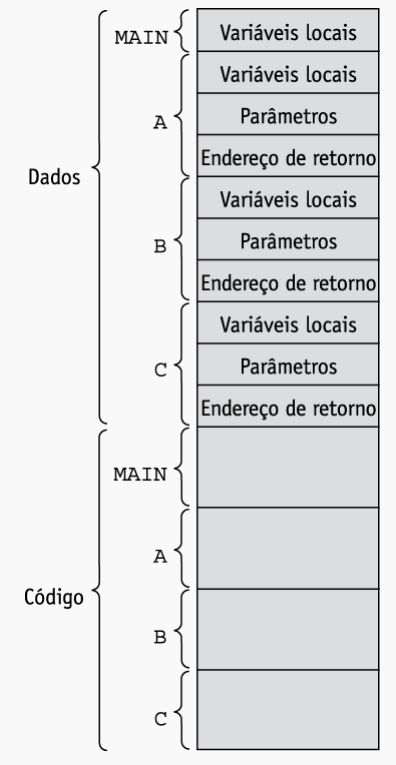
\includegraphics[width=4cm]{img1.png}
    \end{figure}
\end{columns}
\end{frame}
}

\section{Implementando subprogramas com variáveis locais dinâmicas da pilha}

\begin{frame}{Implementando subprogramas com variáveis locais dinâmicas da pilha}
\begin{columns}[T,onlytextwidth]
    \column{0.53\textwidth}
	\begin{itemize}
	\item Registros de ativação mais complexos
	\begin{itemize}
		\item O compilador deve gerar código que faça alocação e liberação implícitas de variáveis locais
		\item Recursão deve ser suportada (adiciona a possibilidade de múltiplas ativações simultâneas de um subprograma)
	\end{itemize}
\end{itemize}
\column{0.53\textwidth}
  \begin{figure}
%\includegraphics[ height=9cm, width=13cm]{figure1.EPS}
  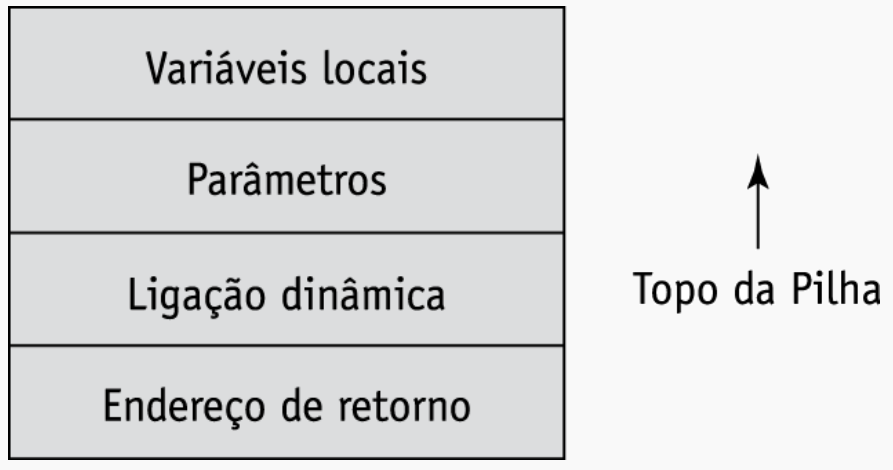
\includegraphics[width=6cm]{fig2.png}
\end{figure}
\end{columns}
\end{frame}

\begin{frame}{Implementando subprogramas com variáveis locais dinâmicas da pilha: registro de ativação}
\begin{itemize}
	\item O formato de um registro de ativação é estático, mas o tamanho pode ser dinâmico
	\item A \textit{ligação dinâmica} é um ponteiro para a base da instância de registro de ativação do chamador
	\item Uma instância de registro de ativação é criada dinamicamente quando um subprograma é chamado
	\item Instâncias de registro de ativação residem na pilha de tempo de execução
	\item O PE (\textit{Environment Pointer}, em inglês) é mantido pelo sistema de tempo de execução. Ele sempre aponta para a base da instância do registro de ativação da unidade de programa que está sendo executada
\end{itemize}
\end{frame}
\begin{frame}{Um exemplo: função C}

\begin{columns}[T,onlytextwidth]
    \column{0.33\textwidth}
	
    	void sub(float total, int part)\{
    
    \hspace{1cm} int list[5];
        
    \hspace{1cm} float sum;
        
    \hspace{1cm} …
        
    \}
	
    \column{0.50\textwidth}
    \begin{figure}
    %\includegraphics[ height=9cm, width=13cm]{figure1.EPS}
      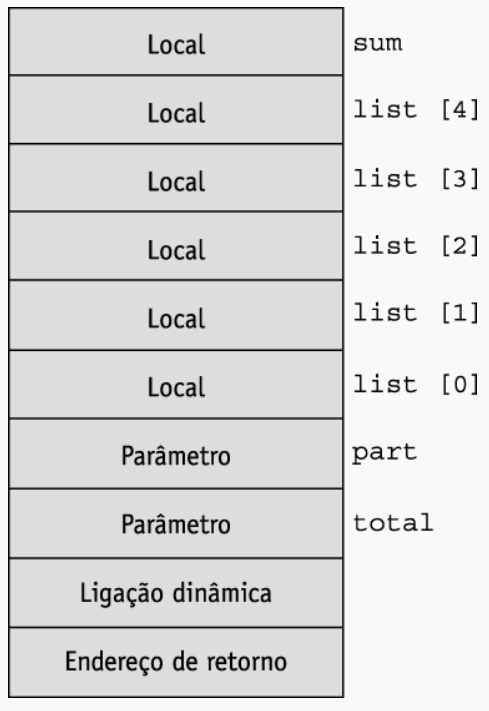
\includegraphics[width=4cm]{img3.png}
    \end{figure}
\end{columns}
\end{frame}


\begin{frame}{Um exemplo sem recursão}

\begin{columns}[T,onlytextwidth]
  \column{0.33\textwidth}
	
    	void A(int x)\{
    
    \hspace{1cm} int y;
        
    \hspace{1cm} …
    
    \hspace{1cm} C(y);
    
    \hspace{1cm} …
    
    \}
	
	void B(float r)\{
    
    \hspace{1cm} int s, t;
        
    \hspace{1cm} …
    
    \hspace{1cm} A(s);
    
    \hspace{1cm} …
    
    \}
    
    void C(int q)\{
    
    \hspace{1cm} …
    
    \}
    
    \column{0.33\textwidth}
    void main()\{
    
    \hspace{1cm} float p;
    
    \hspace{1cm}...
    
    \hspace{1cm}B(p);
    
    \hspace{1cm}...
    
    \}
    
    /*
    
    \hspace{1cm} main chama B
    
    \hspace{1cm} B chama A
    
    \hspace{1cm} A chama C
    
    */
    
    \end{columns}
    
\end{frame}

\begin{frame}{Cadeia dinâmica e deslocamento local}
  
  \begin{figure}
    %\includegraphics[ height=9cm, width=13cm]{figure1.EPS}
      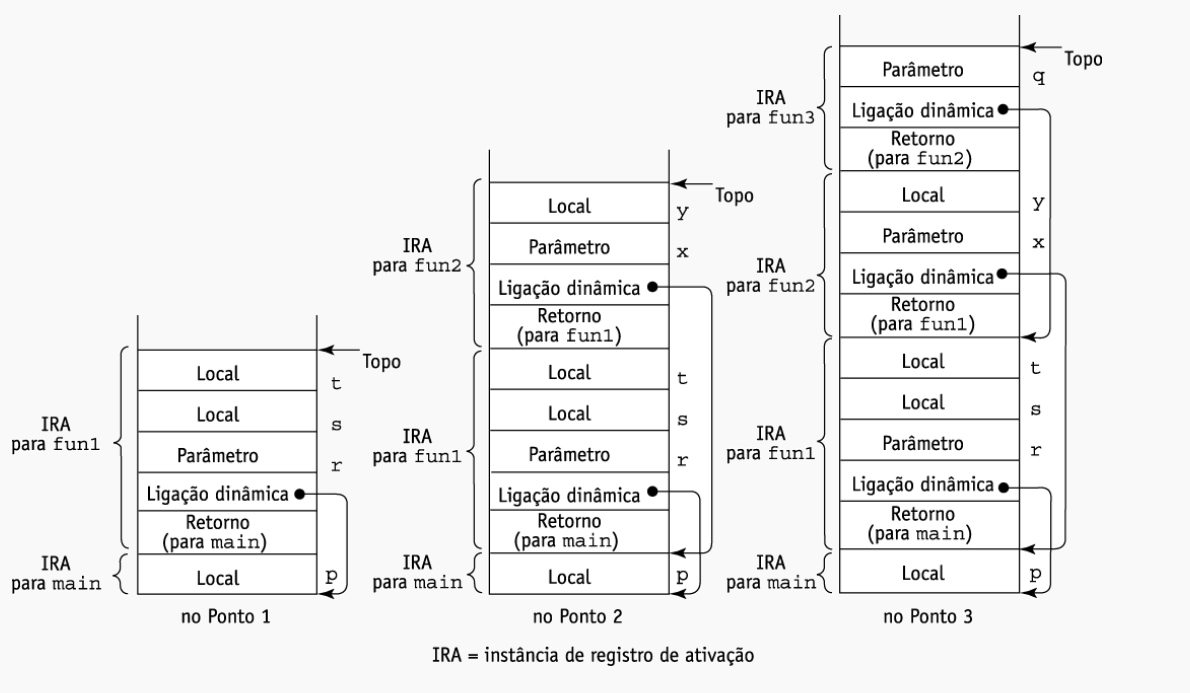
\includegraphics[width=10cm]{img4.png}
    \end{figure}
  
\end{frame}

\begin{frame}{Cadeia dinâmica e deslocamento local}
    \begin{itemize}
    	\item A coleção de ligações dinâmicas presentes na pilha em um dado momento é chamada de \textit{cadeia dinâmica} ou \textit{cadeia de chamadas}
    	\item Referências a variáveis locais podem ser representadas no código como deslocamentos a partir do início do registro de ativação do escopo local, cujo endereço é armazenado no PE. Tal deslocamento é chamado de \textit{deslocamento local (local\_offset)}
    	\item O deslocamento local de uma variável em um registro de ativação pode ser determinado em tempo de compilação
    \end{itemize}

\end{frame}

\begin{frame}{Um exemplo com recursão}
 \begin{itemize}
    	\item Considere o seguinte exemplo de programa em C, que usa recursão para calcular a função fatorial
    \end{itemize}
    
    \begin{columns}[T,onlytextwidth]
    \column{0.60\textwidth}
  
    int factorial(int n)\{
    
    \hspace{1cm} <----------------------------- 1
    
    \hspace{1cm} if (n <= 1)
    
    \hspace{1cm}\hspace{1cm} return 1;
    
    \hspace{1cm} else
    
    \hspace{1cm}\hspace{1cm} return (n * factorial(n  - 1));
    
    \hspace{1cm}<----------------------------- 2
    
    \}
    \column{0.60\textwidth}
    void main() \{
    
    \hspace{1cm} int value;
    
    \hspace{1cm} value = factorial(3);
    
    \hspace{1cm}<----------------------------- 3
    
    \}
    
    \end{columns}
    
\end{frame}
\begin{frame}{O registro da ativação para factorial}
  
  \begin{figure}
    %\includegraphics[ height=9cm, width=13cm]{figure1.EPS}
      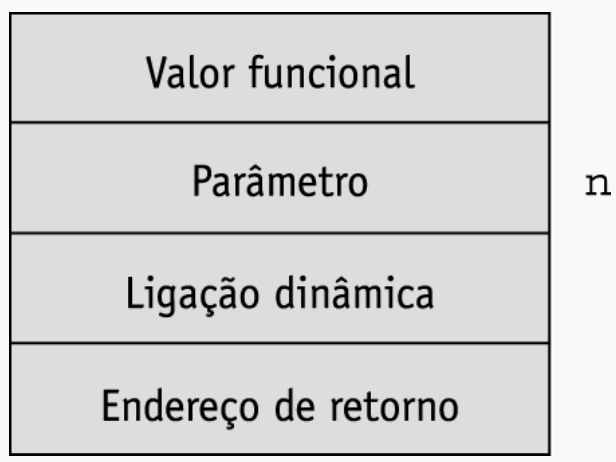
\includegraphics[width=5cm]{img5.png}
    \end{figure}
  
\end{frame}


\section{Subprogramas aninhados}

\begin{frame}{Subprogramas aninhados}
  
  \begin{itemize}
	\item Algumas das linguagens de programação de escopo estático não baseadas em C (Fortran 95, Ada, Python, JavaScript e Lua) usam variáveis locais dinâmicas da pilha e permitem que os subprogramas sejam aninhados
	\item Todas as variáveis não estáticas que podem ser acessadas não localmente estão em instâncias de registro de ativação existentes e, logo, estão em algum lugar na pilha
	\item O processo de referência para uma variável não local:
	\begin{enumerate}
		\item Encontrar a instância de registro de ativação na pilha na qual a variável foi alocada
		\item Usar o deslocamento local da variável (dentro da instância de registro de ativação) para acessá-la
	\end{enumerate}
\end{itemize}
  
\end{frame}

\begin{frame}{Localizar uma referência não local}

\begin{itemize}
	\item Encontrar o deslocamento é fácil
	\item Encontrar a instância de registro de ativação correta
	\begin{itemize}
		\item Regras de semântica estática garantem que todas as variáveis não locais que podem ser referenciadas foram alocadas em alguma instância de registro de ativação que está na pilha quando a referência é feita
	\end{itemize}
\end{itemize}

\end{frame}

\begin{frame}{Encadeamentos estáticos}

\begin{itemize}
	\item Um \textit{encadeamento estático} é uma cadeia de ligações estáticas que conectam certas instâncias de registro de ativação na pilha
	\item A \textit{ligação estática} aponta para o final da instância de registro de ativação de uma ativação do ancestral estático 
	\item A cadeia estática de uma instância de registro de ativação conecta a todos os seus ancestrais estáticos
	\item \textit{Profundidade estática} é um inteiro associado com um escopo estático que indica o quão profundamente ele está aninhado no escopo mais externo
	\item O deslocamento de encadeamento \textit{(chain\_offset)} ou profundidade de aninhamento \textit{(nesting\_depth)} de uma referência não local é a diferença entre a profundidade estática do procedimento que contém a referência a x e a profundidade estática do procedimento contendo a declaração de x
	\item A referência à variável pode ser representada por: (chain\_offset, local\_offset),
\end{itemize}

\end{frame}

\begin{frame}{Exemplo de Programa em Ada}
 \begin{columns}[T,onlytextwidth]
    \column{0.60\textwidth}
    \begin{figure}
        %\includegraphics[ height=9cm, width=13cm]{figure1.EPS}
          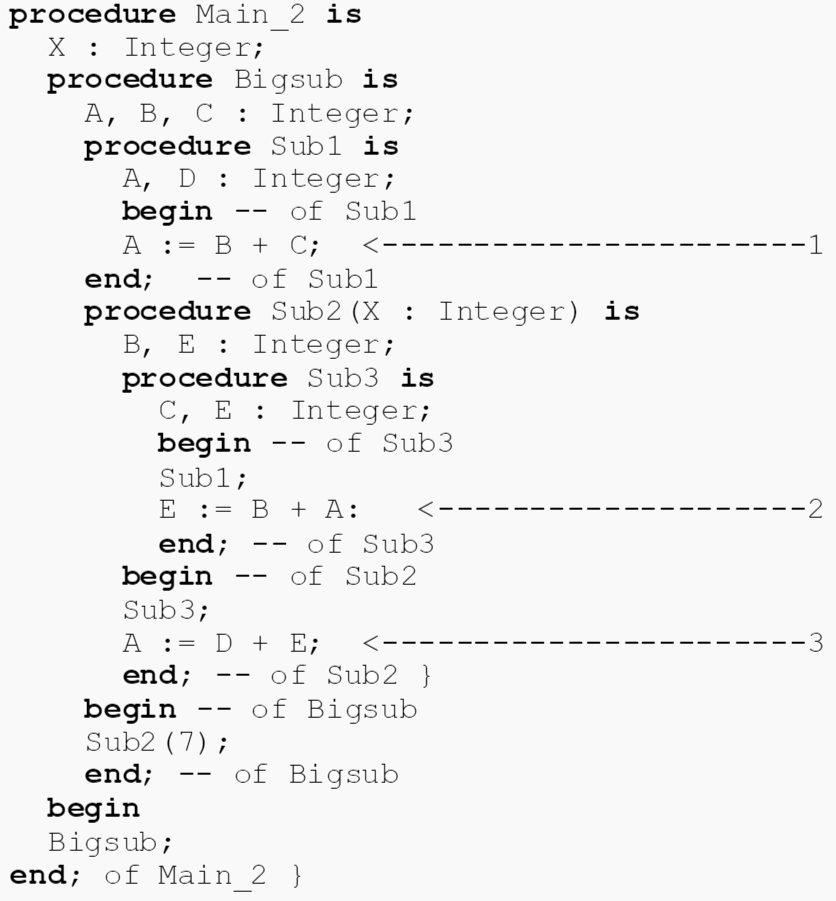
\includegraphics[width=7cm]{img6.png}
        \end{figure}
    \column{0.60\textwidth}
        \begin{itemize}
    	    \item A sequencia de chamada a procedimentos é:
        \end{itemize}
        \hspace{1cm} Main\_2 \textbf{chama} Bigsub
        
        \hspace{1cm} Bigsub \textbf{chama} Sub2
        
        \hspace{1cm} Sub2 \textbf{chama}  Sub 3
        
        \hspace{1cm} Sub3 \textbf{chama} Sub1
    
\end{columns}
\end{frame}

\begin{frame}{Conteúdo da pilha na posição 1 do programa}
\begin{figure}
        %\includegraphics[ height=9cm, width=13cm]{figure1.EPS}
          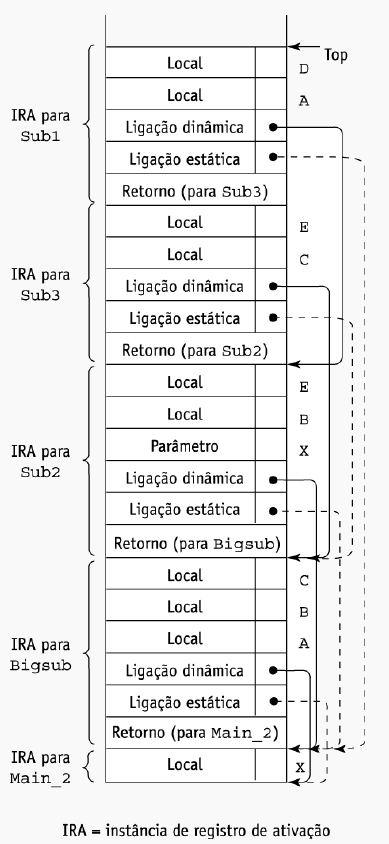
\includegraphics[width=3.5cm]{fig7.png}
        \end{figure}

\end{frame}

\begin{frame}{Manutenção de cadeias estáticas}

\begin{itemize}
	\item No momento da chamada,
	\begin{itemize}
	    \item A instância de registro de ativação deve ser encontrada
	    \item \textcolor{red}{The dynamic link is just the old stack top pointer}
	    \item \textcolor{red}{The static link must point to the most recent ari of the static parent}
	    \begin{itemize}
	    \item Dois métodos
	    \begin{enumerate}
	    \item Busca a cadeia dinâmica
	    \item Trata chamadas a subprogramas e definições como referências variáveis e definições
	    \end{enumerate}
	    \end{itemize}
	\end{itemize}
\end{itemize}

\end{frame}

\begin{frame}{Avaliação de cadeias estáticas}

\begin{itemize}
	\item Problemas: 
	\begin{enumerate}
	    \item Uma referência não local é lenta se a profundidade de aninhamento é grande
	    \item Código com tempo limitado é difícil:
	    \begin{itemize}
            \item Custos de referências não locais são difíceis de determinar
            \item Mudanças de código podem mudar a profundidade de aninhamento
        \end{itemize}
	\end{enumerate}
\end{itemize}

\end{frame}


\begin{frame}{Mostradores (\textit{displays})}

\begin{itemize}
	\item Uma alternativa ao encadeamento estático que resolve os problemas com essa abordagem
	\item Ligações estáticas são armazenadas em uma única matriz chamada mostrador (display)
	\item O conteúdo do mostrador em um determinado momento é uma lista de endereços das instâncias de registro de ativação
\end{itemize}

\end{frame}

\section{Blocos}

\begin{frame}{Blocos}
\begin{itemize}
	\item Blocos são escopos locais especificados pelo usuário para variáveis
	\item Um exemplo em C
\end{itemize}
\{

int temp;

temp = list [upper];

list [upper] = list [lower];

list [lower] = temp

\}
\begin{itemize}
	\item O tempo de vida de \textit{temp} no exemplo começa quando o controle entra no bloco
	\item A vantagem de usar tal variável local é que ela não pode interferir com outras variáveis com o mesmo nome que são declaradas em outros lugares do programa
\end{itemize}

\end{frame}

\begin{frame}{Implementando blocos}
\begin{itemize}
	\item Dois métodos
	\begin{enumerate}
	    \item Blocos são tratados com o subprogramas sem parâmetros que são sempre chamados a partir do mesmo local do programa
	    \begin{itemize}
	        \item Cada bloco tem um registro de ativação; uma instância é criada a cada vez que o bloco é executado
	   \end{itemize}
	   \item Já que o máximo de armazenamento necessário para um bloco pode ser determinado, esse espaço pode ser alocado depois das variáveis locais no registro de ativação
	\end{enumerate}
\end{itemize}

\end{frame}

\section{Implementando escopo dinâmico}

\begin{frame}{Implementando escopo dinâmico}
\begin{itemize}
	\item \textit{Acesso profundo}: as referências a variáveis não locais podem ser resolvidas com buscas por meio das instâncias de registros de ativação dos subprogramas ativos
	\begin{itemize}
        \item O tamanho da cadeia não pode ser estaticamente determinado
        \item Os registros de ativação devem armazenar os nomes das variáveis
    \end{itemize}
    \item \textit{Acesso raso}: coloca as variáveis locais em uma tabela central
    \begin{itemize}
        \item Uma pilha separada para cada nome de variável
        \item Tabela central com entrada para cada nome de variável
    \end{itemize}
\end{itemize}

\end{frame}


\begin{frame}{Usando acesso raso para implementar escopo dinâmico}
\begin{figure}
        %\includegraphics[ height=9cm, width=13cm]{figure1.EPS}
          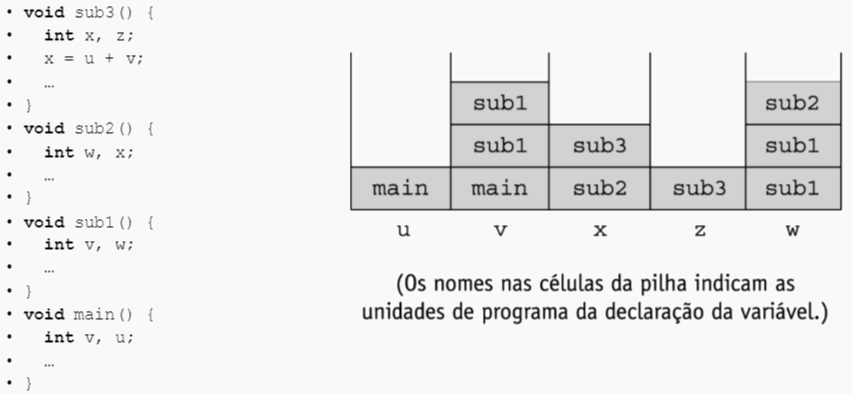
\includegraphics[width=10.5cm]{img8.png}
        \end{figure}


\end{frame}

\begin{frame}{Resumo}
\begin{itemize}
	\item A semântica de ligação de subprogramas requer muitas ações por parte da implementação
	\item No caso de subprogramas "simples", essas ações são relativamente básicas
	\item Linguagens dinâmicas da pilha são mais complexas
	\item Subprogramas em linguagens com variáveis locais dinâmicas da pilha e subprogramas aninhados têm dois componentes
	\begin{itemize}
        \item código real
        \item registro de ativação
    \end{itemize}
    \item \textit{Acesso raso}: coloca as variáveis locais em uma tabela central
    \begin{itemize}
        \item Uma pilha separada para cada nome de variável
        \item Tabela central com entrada para cada nome de variável
    \end{itemize}
\end{itemize}

\end{frame}

\begin{frame}{Resumo (continuação)}
\begin{itemize}
	\item Instâncias de registro de ativação contêm os parâmetros formais e as variáveis locais, dentre outras coisas
	\item A ligação estática é usada para permitir referências para variáveis não locais em linguagens de escopo estático
	\item O acesso às variáveis não locais em uma linguagem de escopo estático pode ser implementado pelo uso de encadeamento dinâmico ou por meio de algum método de tabela variável central
\end{itemize}

\end{frame}

\end{document}
